%author: alhelal
%date: 03.09.19
\documentclass[a4paper, 12pt]{article}
\usepackage[utf8]{inputenc}
\usepackage{fullpage, graphicx, tikz, float, advdate}
\usetikzlibrary{shapes,arrows}
\usepackage{biblatex}
\addbibresource{../bibliography.bib}



\begin{document}
\begin{titlepage}
\centering

\includegraphics[width=7cm,height=4cm]{Image/dulogoblue.jpg}\\
{\scshape\LARGE University of Dhaka \par}
\vspace{1cm}
{\scshape\Large Course: Zool.110\par}
\vspace{1.5cm}
{\huge\bfseries A Report on Insects in the Bangladesh National Zoo\par}
\vspace{2cm}
{}
\vfill
Submitted by - \\
\vspace{0.5cm}
Md. Al- Amin Shuvo\\ Roll: 1213\\Reg. No.:2018-426-070\\Session: 2018-19
\vfill
% Bottom of the page
\SetDate[01/12/2019]
{\large \today\par}
\end{titlepage}



%\title{Humanoid Robot Behavior Generation to Improve Social Skill of Autistic Children}
%for ICT ministry scholarship
%\author{Md. Al-Helal \\ supervisor: Dr. Saifuddin Md. Tareeq,\\Professor\\Department of Computer Science \& Engineering,\\University of Dhaka}
%\date{September 12, 2019}

%\begin{document}

%\maketitle
\newpage
\tableofcontents
\newpage
\section{Objective}
Observation of various kinds of animals to gain first-handed experience and knowledge.
\section{Abstract}
Insect is the largest group of arthropods found in both land and water all around the world.As student of zoology i am fascinated by their morphological diversity. Acquiring practical knowledge is a must for all student of zoology. With this vision, a field trip was arranged by arranged by Department of Zoology, University of Dhaka to the Bangladesh National Zoo.
\section{Introduction}
Bangladesh National Zoo is located at Mirpur in Dhaka. This is the largest zoo in Bangladesh, and is run by the Ministry of Fisheries \& Livestock. The zoo contains many native and non-native animals and wild life, and hosts about four million visitors each year. The zoo is currently holding home to 2799 animals from 138 species. The zoo exhibits 46 species of mammals, including elephants, cheetah, rhinos, zebras, water-bucks, otters, giraffes, impala, black bears, tapirs, hippos, lions, many species of monkeys, chimpanzees, baboons, \& the Royal Bengal Tigers. The aviaries at the zoo house more than 1196 birds representing 57 species, including peacocks, rhea, African gray parrots, cassowary, owls, ostrich, emus, teals, finches, babblers, owls, vultures, and
eagles. The two lakes at the zoo also host migratory water birds each winter. Visitors can also see 9 species of reptiles including snakes and crocodiles and 26 species of fish.
\section{Insect}
Insects, are a class in the phylum Arthropoda.They are small terrestrial invertebrates which have a hard exoskeleton. Insects are the largest group of animals on earth by far: about 926,400 different species have been described.They are more than half of all known living species.They may be over 90\% of animal species on Earth.New species of insects are continually being found.Estimates of the total number of species range from 2 million to 30 million.Insects have hard skeletons are made out of thin, hard pieces or plates, like armour, made of chitin.The body of an insect has three main parts: a head, a thorax, and an abdomen. On the head are an insect’s compound eyes, its two antennae and its mouth.On the thorax, insects have wings and legs. All insects have six legs and usually four wings.The abdomen is the back part of the insect. Inside the abdomen is the stomach, the heart, and the excretory system where body wastes pass out of the insect. Bees also have a stinger at the back of the abdomen. Insects are cold-blooded, which means that they cannot control their body temperature.Insects are not good at surviving the cold. In the winter, many insects go into something called diapause, which is the insect version of hibernation.Insects are adapted to every land and freshwater habitat where food is available, from deserts to jungles, from glacial fields and cold mountain streams to stagnant, lowland ponds and hot springs. Many live in brackish water up to 0.1\% the salinity of seawater, a few live on the surface of seawater, and some fly larvae can live in pools of crude petroleum, where they eat other insects that fall in.
\section{Observation}
\begin{enumerate}
\item Grasshopper\\

\begin{figure}[H]
\centering
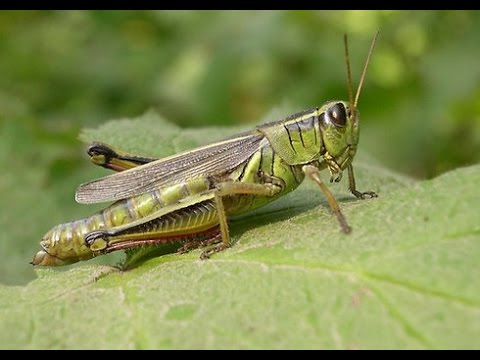
\includegraphics[scale=0.5]{Image/hqdefault.jpg}
\caption{Grasshopper}
\end{figure}
\begin{tabular}{lcl}
Animal count     &:& 11\\
Distribution     &:& Worldwide\\
Diet             &:& Herbivore \\
Scientific name  &:& \textit{Caelifera}
\end{tabular}
\item Water strider\\
\begin{figure}[H]
\centering
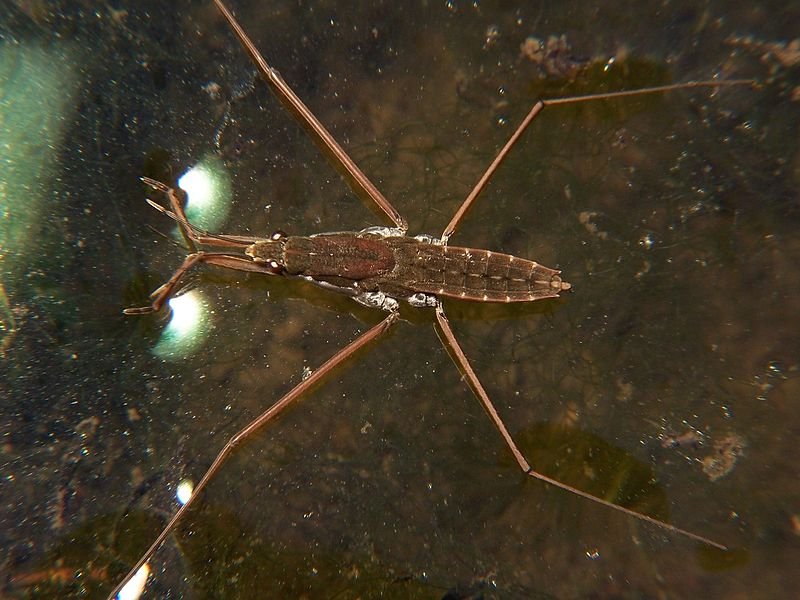
\includegraphics[scale=0.3]{Image/800px-Water_strider_G_remigis.jpg}
\caption{Water strider}
\end{figure}
\begin{tabular}{lcl}
Animal count     &:& 23\\
Distribution     &:& Any pond, river, or lake\\
Common name      &:& water skeeters, water bugs\\
Scientific name  &:& \textit{Gerridae}
\end{tabular}

\item Ladybug\\
\begin{figure}[H]
\centering
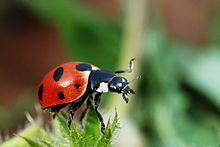
\includegraphics[scale=4]{Image/220px-Coccinella_magnifica01.jpg}
\caption{Ladybug}
\end{figure}
\begin{tabular}{lcl}
Animal count     &:& 8\\
Distribution     &:& Grassland areas,forest,woodland\\
Diet             &:& Honeydew, pollen, plant sap, nectar\\
Scientific name  &:& \textit{Coccinellidae}
\end{tabular}

\item Dung beetle\\
\begin{figure}[H]
\centering
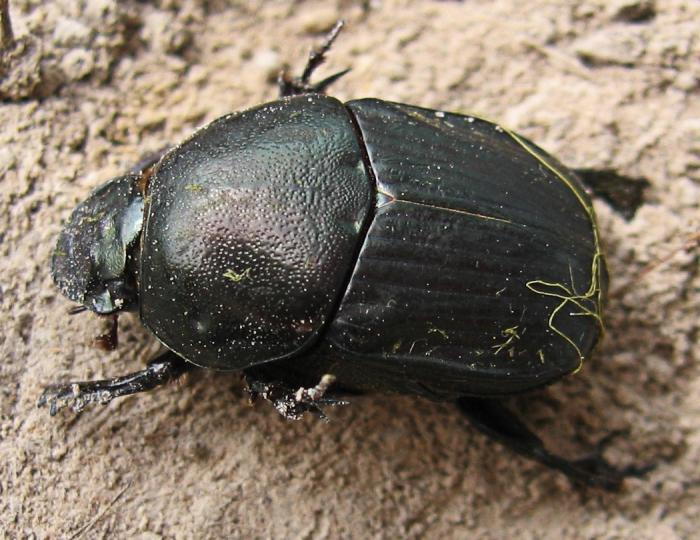
\includegraphics[scale=0.3]{Image/fjskdfsafhak.jpg}
\caption{Dung beetle}
\end{figure}
\begin{tabular}{lcl}
Animal count     &:& 4\\
Distribution     &:& Desert, grasslands and savannas\\
Diet             &:& Herbivore\\
Scientific name  &:& \textit{Scarabaeus}
\end{tabular}
\item Black garden ant\\
\begin{figure}[H]
\centering
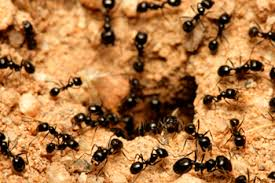
\includegraphics[scale=0.75]{Image/blackants.jpeg}
\caption{Black garden ant}
\end{figure}
\begin{tabular}{lcl}
Animal count     &:& many\\
Distribution     &:& Europe,in some parts of America, Asia and Australasia\\
Diet             &:& Herbivore\\
Scientific name  &:& \textit{Lasius niger}
\end{tabular}
\item Bengal dark evening brown Butterfly\\
\begin{figure}[H]
\centering
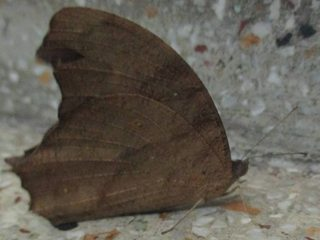
\includegraphics[scale=0.7]{Image/brownbutterflies.jpg}
\caption{Bengal dark evening brown Butterfly}
\end{figure}
\begin{tabular}{lcl}
Animal count     &:& 7\\
Distribution     &:& India,Bangladesh,Myanmar,Thailand\\
Diet             &:& Herbivore\\
Scientific name  &:& \textit{Melanitis phedima bela}
\end{tabular}
\end{enumerate}
\newpage
\section{Conclusion}
Bangladesh National Zoo is a place where people from all parts of out society can learn about animals and enjoy the wonders of the nature. It can also be a research center for students and researchers. However, lack of proper training, management, manpower and the negligence from the government high ups has turned the zoo into a death camp for animals. If the pending renovation project comes into light there is a hope that it will be one of the most tourist attraction sites in Bangladesh and a conservation center of international standards.
\end{document}
